\documentclass{article}
\usepackage[utf8]{inputenc}

\usepackage[english]{babel}
\usepackage[utf8]{inputenc}
\usepackage{amssymb, amsmath}
\usepackage{amsfonts}       % blackboard math symbols
\usepackage[round]{natbib}
\usepackage{graphicx}
\usepackage{subfig}
\usepackage[colorinlistoftodos]{todonotes}
\usepackage{lineno, a4wide}
\usepackage{hyperref}
\usepackage{xcolor}
\usepackage{subfiles}
\usepackage{parskip}
\usepackage{multirow}
\usepackage{doi}
\usepackage{times}
\usepackage[para,online,flushleft]{threeparttable}
\usepackage{rotating}
\usepackage{tikz}
\usepackage{tcolorbox}

\linenumbers

\title{Estimating the zone of influence and cumulative anthropogenic footprint of infrastructures on animal space use \\
{\normalsize in preparation for \textit{Journal of Applied Ecology}}}
\author{B. Van Moorter, M. Panzacchi, A. Moudud, A. Skarin, B.B.S. Niebuhr, \\ O. Strand, K. Langeland, T. Tveraa, A. Stien}
\date{\today}

\begin{document}
\maketitle

\begin{abstract}
We compare distance and density and do the math to compute the zone of influence and footprint for anthropogenic infrastructures. 
\end{abstract}


\section{Introduction}

Maps of human influence or `human footprint'\footnote{The `human footprint' is not to be confused with the `ecological footprint', which measures the impact of a person or community on the environment as the amount of land required to sustain their use of natural resources.} are commonly used to identify wilderness areas relatively free of such influences \citep{sanderson2002human,allan2017temporally}. These maps are increasingly used in global analyzes of effects of human activities on biodiversity \citep{tucker2018moving,williams2020change}. The human footprint integrates into a single index different types of human influence, such as urban areas, roads, railway, power lines, forestry, mining, hydropower reservoirs, etc. \citep{woolmer2008rescaling}. Hence, this represents the structural footprint of human activities, but does not address the different effects from those activities on ecosystems. In this study, we propose a method to quantify the anthropogenic footprint of each human activity separately and cumulative on ecosystems, we illustrate our approach with the human footprint on space use of the tundra's flagship species, reindeer.  

While human activities and infrastructures may have an immediate effect where they are located, i.e. their structural footprint (see Box with definitions), their actual effect or functional footprint on an ecosystem often cover a much larger zone of influence (ZoI), for some species many kilometers away from the actual infrastructure \citep{torres2016assessing}. Not surprising, estimating the ZoI of an infrastructure on ecosystems is crucial for environmental impact assessments. In estimating ZoI, the concept of ecological threshold \citep{holling1973resilience} and analytical procedures developed therein \citep{ficetola2009ecological} are used \citep{boulanger2012estimating}. Under this framework, the estimation of the zones of influence is often carried out by fitting piece-wise regression models \citep{ficetola2009ecological} or other non-linear functions \citep[such as an exponential decay;][]{skarin2018out} to the measured response of an ecosystem to an infrastructure as a function of distance. This distance is typically the distance to the nearest instance of this infrastructure type, ignoring potential additive or cumulative effects of multiple instances or features of an infrastructure.   

Piecemeal development also called 'nibbling' is the type of cumulative impact, where a single feature may have a negligible effect but multiple features together may have a substantial effect on an ecosystem \citep{nellemann2003progressive}. For instance, a single cabin will have no discernible effect on reindeer habitat and space use, however an area with many cabins will be avoided resulting in habitat loss. Exclusive focus on the nearest feature of an infrastructure fails to address such cumulative effects from multiple features. 

In this study, we first develop a formal framework to quantify simultaneously the ZoI and the cumulative impact of multiple features, which we then illustrate for houses and private cabins on summer space use of the largest reindeer herd in Norway. Finally, we demonstrate the computation of the different types of footprints for these infrastructures.  

\begin{tcolorbox}[colback=yellow!5,colframe=yellow!75!black,title=BOX -- Types of Anthropogenic Footprint]
\begin{itemize}
    \item The \textbf{structural footprint} is the physical space directly affected by an infrastructure, whereas the \textbf{functional footprint} -- the focus of our study -- is the effect of an infrastructure on a given ecosystem component.  
    \item The \textbf{theoretical footprint} of an infrastructure combines it's zone of influence and it's effect size. 
    \item The prediction of the theoretical footprint for the features of an infrastructure's present in the landscape gives it's \textbf{potential footprint}.
    \item The imprint of the potential footprint onto the natural suitability of an area's habitat is the \textbf{realized footprint} of an infrastructure. In other words, the realized footprint in an area is high, when the habitat is suitable and the potential footprint is high.  
    \item The (theoretical/potential/realized) footprint of different infrastructures can be combined to quantify their \textbf{cumulative footprint}. 
\end{itemize}
\end{tcolorbox}


\section{Method}
\subsection{Deriving the estimation of the cumulative impact of multiple features}

% For tables use
\begin{table}
% table caption is above the table
\caption{Symbols used in the paper}
\label{tab:symbols} % Give a unique label
% For LaTeX tables use
\begin{threeparttable}
\begin{tabular}{ll}
\hline\noalign{\smallskip}
Symbol & Meaning\tnote{1} \\
\noalign{\smallskip}\hline\noalign{\smallskip}
$k$ & infrastructure type $k$ \\
$i_k$ & feature $i$ of infrastructure type $k$ ordered by increasing distance from the current location, $i \in [1;n_k]$ \\
$\Delta_{i_k}$ & distance from the current location to feature $i_k$ \\
ZoI & zone of influence as a distance from $i_k$, also denoted with $\zeta_k$ \\
$\zeta_k$ & zone of influence of an infrastructure type $k$ as a distance from $i_k$ \\
$U$ & use of the current location\\
$\Lambda^T_k$ & theoretical footprint of infrastructure $k$ \\
$\Lambda^P_k$ & potential footprint of infrastructure $k$  \\
$\Lambda^R_k$ & realized footprint of infrastructure $k$  \\
$\beta_{i,k}$ & effect size of feature $i$ of infrastructure type $k$  \\
$\phi_{i_k}$ & influence of feature $i_k$ of infrastructure type $k$: $\phi_{i_k} = 1$, when $\Delta_{i_k} = 0$ and $\phi_{i_k} \simeq 0$, when $\Delta_{i_k} > \zeta_k$  \\
\noalign{\smallskip}\hline
\end{tabular}
\begin{tablenotes}
\item[1] See main text for further details
\end{tablenotes}
\end{threeparttable}
\end{table}

We first derive the cumulative impact of multiple features of an infrastructure type, e.g.\ cabins, on space use.
Let the influence of a feature (i) of an infrastructure (k) be: $\phi_{i_k} = f(\Delta_{i_k}; \zeta_k)$, where $\Delta_{i_k}$ is the distance to a feature ($i_k$) of infrastructure type $k$ and $\zeta_k$ is its zone of influence (see Figure~\ref{fig:ZoI_shapes}).

If there are $n$ features in the landscape, such as cabins, then we can sum the effect of each house on animals space use ($U$):

\begin{equation}
    U = \exp(\sum_{i=1}^{n_k} \beta_{i_k} \phi_{i_k})
\end{equation}

Typically, only the nearest feature is considered, resulting in the implicit assumption that $\beta_i = 0$ for all $i > 1$ (where the features are ordered by increasing distance).

However, possibly a more reasonable assumption would be that  $\beta_i = \beta_{i+1} = \beta_{i+...} = \beta$, i.e. that all $\beta$'s are identical, thus:

\begin{equation}
    U = \exp(\beta \sum_{i=1}^{n_k} \phi_{i_k})
\end{equation}

where $\sum_{i=1}^{n_k} \phi_{i_k}$ is equivalent to what has been called the `density' of a feature \citep[e.g.][]{panzacchi2015searching}.

Analogous to \citet{lee2020estimating}'s recasting of the identification of the ZoI of a single (i.e. the nearest) infrastructure as a model selection rather than a parameterization problem, we can also estimate the ZoI and cumulative effect of features using model selection. 

\subsection{Empirical demonstration}

For our empirical demonstration we used GPS tracking data from the Hardangervidda reindeer population in Southern Norway, which is the largest population of wild mountain reindeer in Europe. We used data from XXX individuals during the summer season \citep[see][for further details]{panzacchi2015searching}.
To account for bio-climatic-geographical variation in environmental characteristics we used the four components from a large principal component (PC) analysis conducted for Norway \citep{bakkestuen2008step}, which correspond to: (1) PC1 - continentality, (2) PC2 - altitude, (3) PC3 - ruggedness, and (4) PC4 - solar radiation; we included a quadratic term for PC1 and PC2. We used the SatVeg map with 21 vegetation classes, which we further grouped (see Table~\ref{tab:model_results}). To keep model fitting relatively simple we included two anthropogenic variable: private and tourist cabins, for which we estimated the cumulative effects and footprint. There are a total of 13,015 private cabins compared to only 26 tourist cabins within the study area. Furthermore, we did not perform model selection, but compared models based on different representation of the influence of private cabins.

We estimated the effect of both private and tourist cabins for 8 ZoI: 100, 250, 500, 1000, 2500, 5000, 10000, and 20000 meter. For each ZoI, we used three shapes for the changing effect over the ZoI (see Figure~\ref{fig:ZoI_shapes}): threshold, linear decline, and half-normal ($\phi_{i_k} = \exp(-2.77(\Delta_{i_k}/\zeta_k)^2)$), and two assumptions for the effect of additional features (see Figure): $\beta_i \neq 0$ for $i=1$ and $\beta_i = 0$ for all $i > 1$ (i.e.~only the nearest feature has an effect) versus $\beta_i = \beta$ for all $i$ (i.e.~all features contribute to a cumulative effect). With all combinations, we fitted a total of 2304 (i.e. $(8 \times 3 \times 2)^2$) RSFs. The RSFs were fitted using the {\tt survival} library in R \citep{therneau2020package, therneau2000modeling}, we selected the best model based on AIC. We then used 99 bootstraps to estimate the standard errors for this model. Note that the ZoI is not well defined for functions with an infinite domain, such as the Gaussian. We therefore linked to ZoI to the function's half-life (i.e. where the influence has halved), thus the half-life of the Gaussian function corresponded to half the distance of the ZoI as it is for the linear shape (the influence at the ZoI has then dropped to $1/16 \approx 0.06$; we computed the influence until 2.55 $\times$ the half-life, when it has dropped further to $e^{-4.5} \approx 0.01$).  

\begin{figure}
\centering
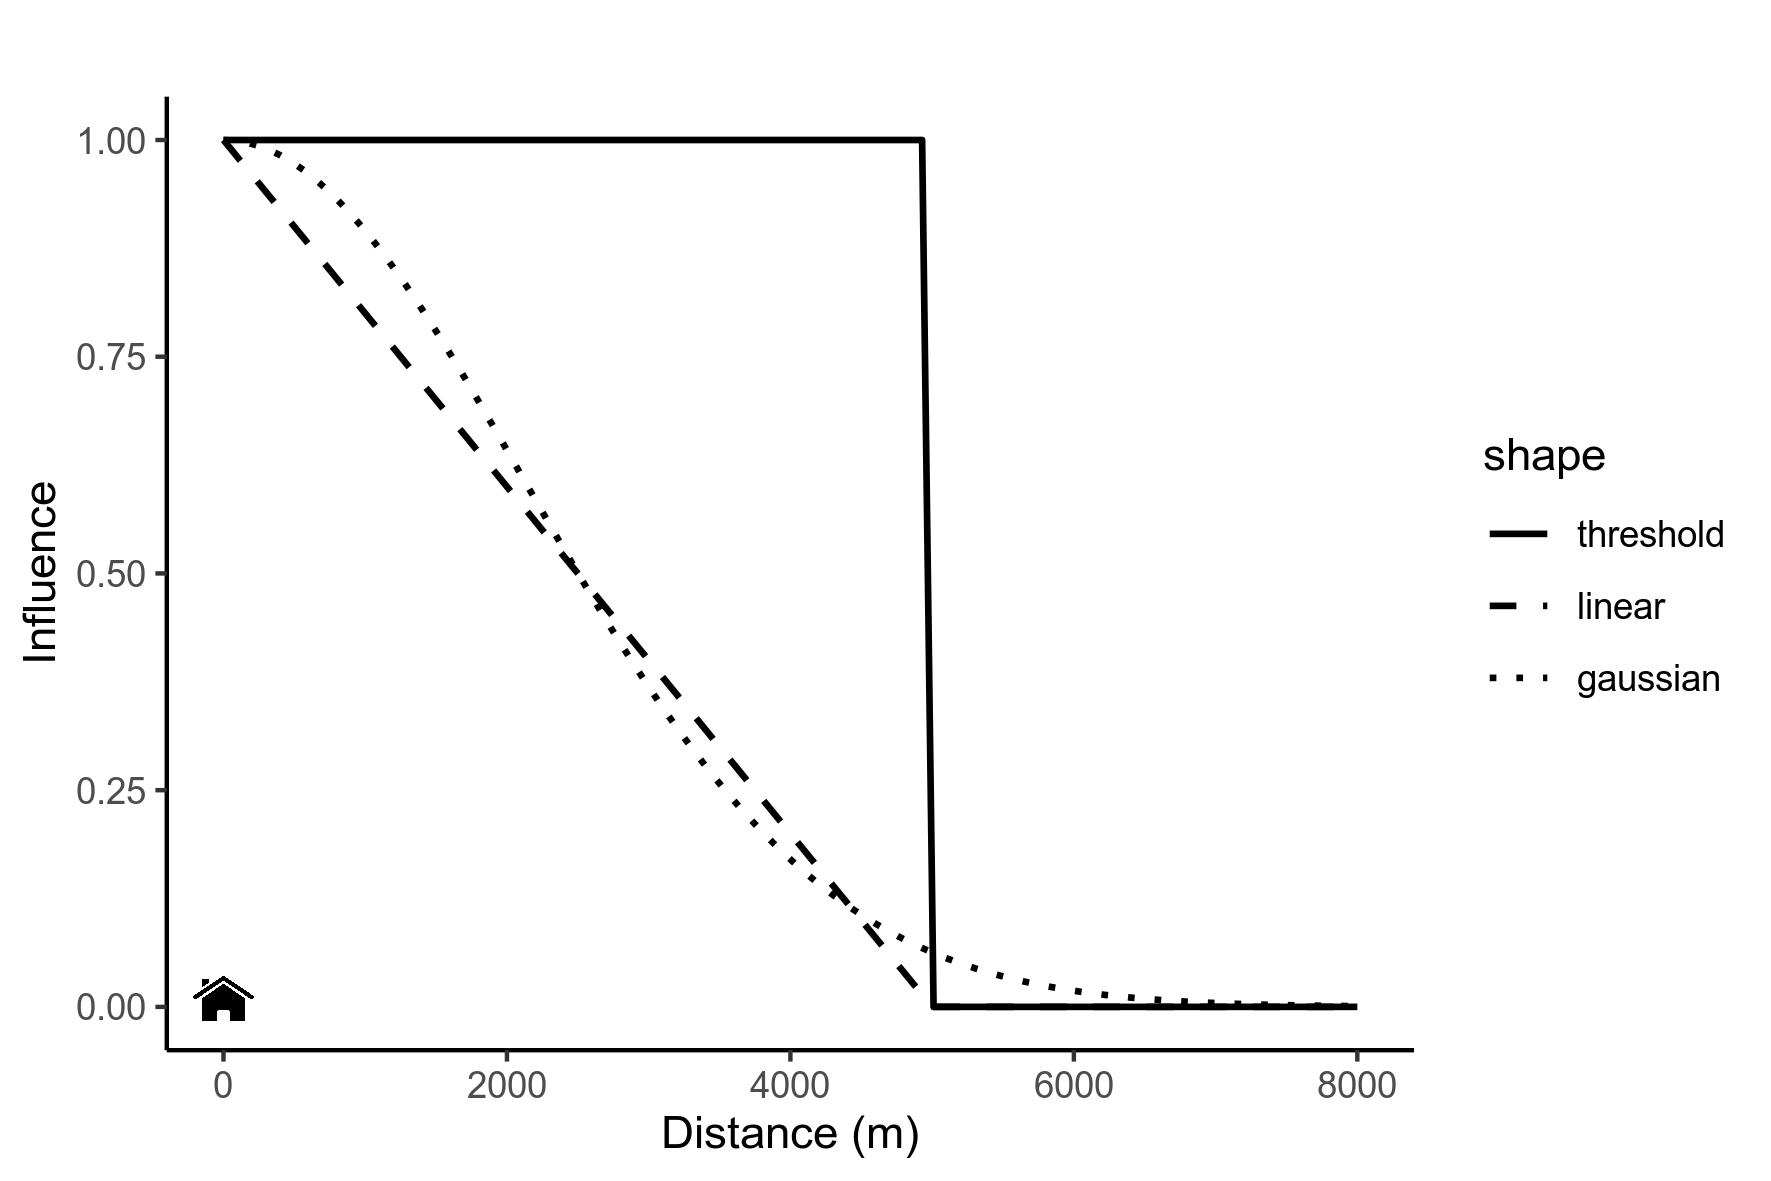
\includegraphics[width=0.9\textwidth]{figures/ZoI_shapes.jpg}
\caption{\label{fig:ZoI_shapes} The influence of a cabin against the distance from the cabin. A cabin has only an influence with in the zone of influence (here the $ZoI=5,000$), and the change in influence within the ZoI can have different shapes. For influence remains constant within the ZoI for the threshold and drops to zero outside, whereas both the linear and Gaussian shapes decline monotonically within the ZoI. Note that for shapes with an infinite domain the ZoI will not be well defined (we therefore defined the ZoI based on the half-life).}
\end{figure}

\begin{figure}
\centering
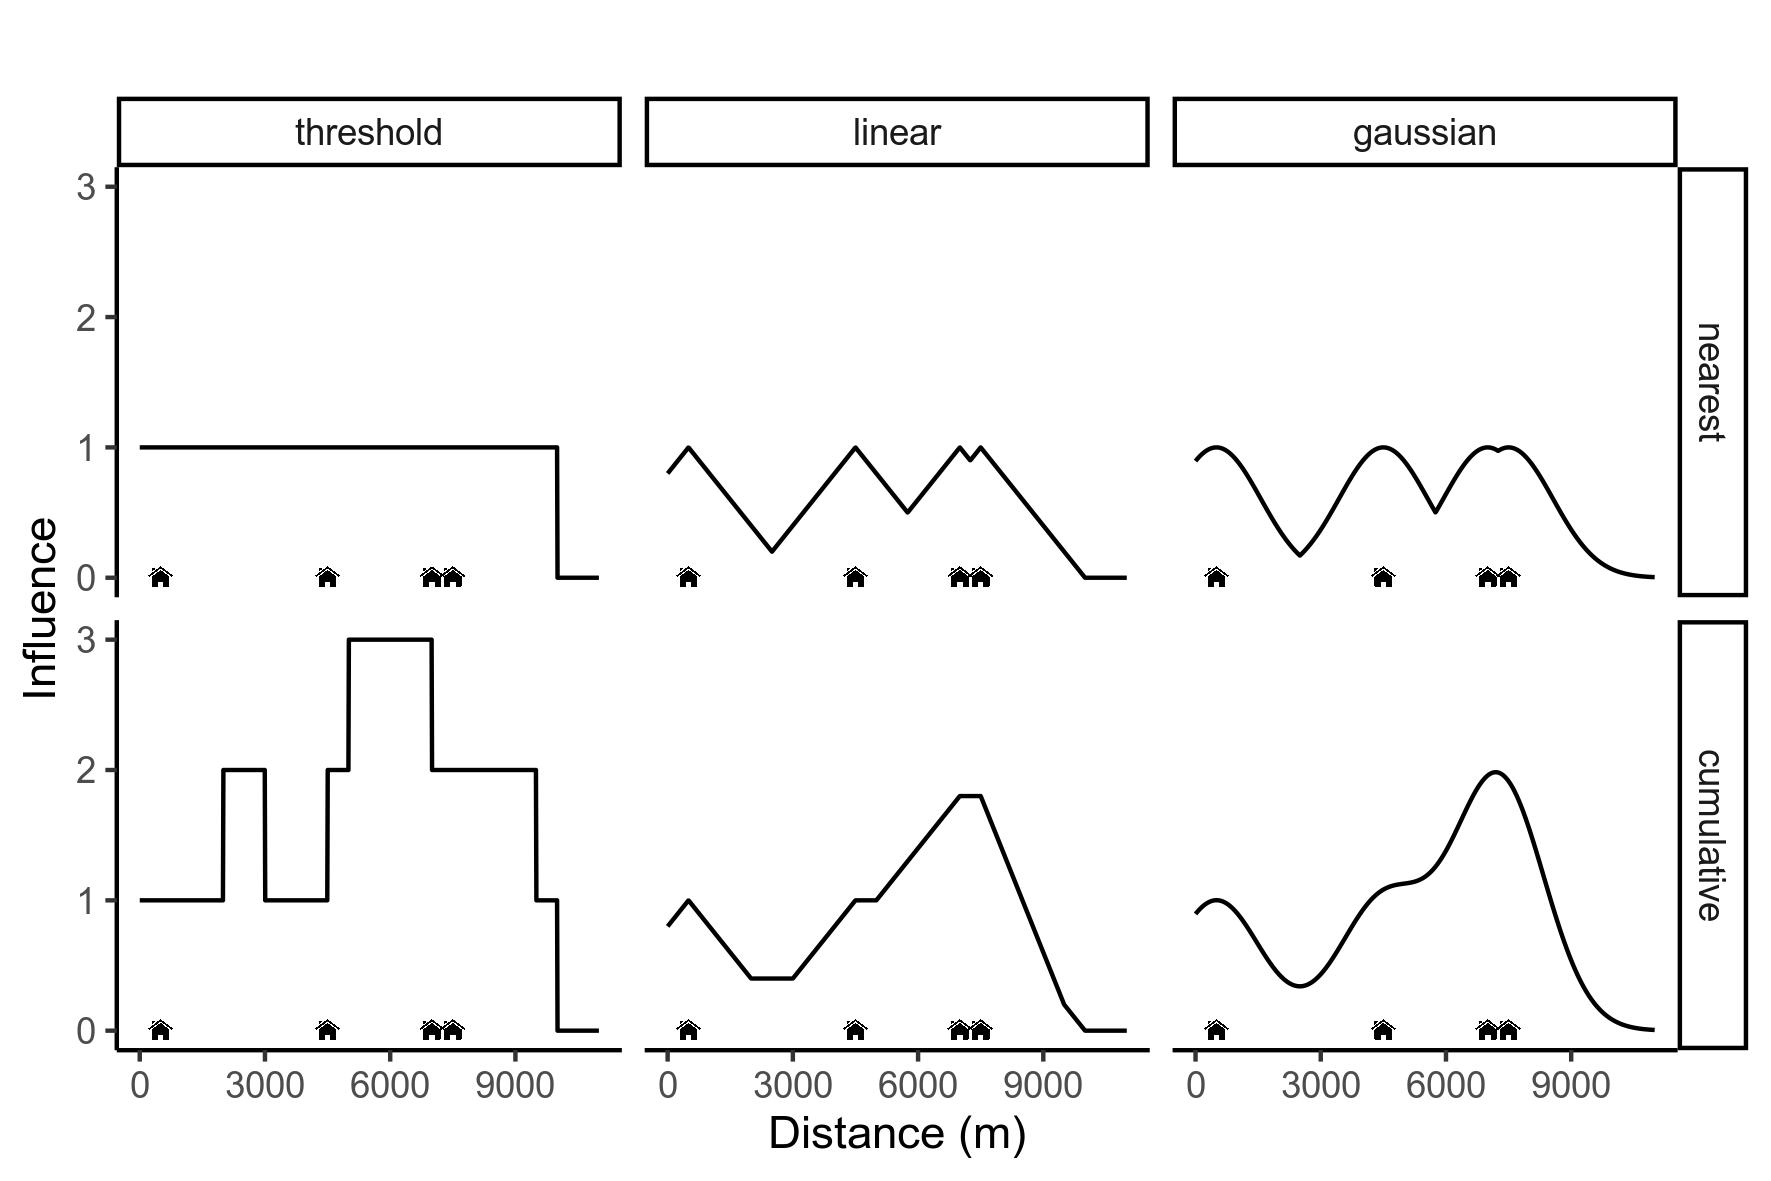
\includegraphics[width=0.9\textwidth]{figures/ZoI_density.jpg}
\caption{\label{fig:ZoI_density} The influence of cabins when only the nearest cabins matters or when all cabins act cumulatively for the three shapes (threshold, linear, and Gaussian). If only the nearest cabin affects space use, the influence will not go above one; whereas, when all cabins act cumulatively, their cumulative effect can be much higher than one.}
\end{figure}

\subsection{Estimating the human footprint}

Finally, we computed the footprint for both private and public cabins from our best model. We computed both the theoretical footprint of a single feature, and the potential and realized footprints for our study area. The theoretical footprint ($\Lambda^T$) is derived by integrating over the ZoI the shape of the distance decay ($V$) with the estimated effect size ($\beta$) from the RSF:

\begin{equation}
    \Lambda^T = \iint\limits_{ZoI} 1-\exp(\beta V_{x,y})
\end{equation}

In addition, the potential footprint ($\Lambda^P$) of an infrastructure for a given study area is obtained by integrating the footprints of all features ($i: 1 \rightarrow n$) of this infrastructure type over the study area ($\Omega$):

\begin{equation}
    \Lambda^P = \iint\limits_{\Omega} 1-\exp(\sum_{i=1}^n \beta_i V_{i,x,y})
\end{equation}

Whereas, the realized footprint ($\Lambda^R$) is the effect of the potential footprint on the `natural' suitability. I.e. an infrastructure may have a large potential footprint, but when this footprint does not overlap with suitable habitat ($S(H)$), it will not have a large realized footprint:

\begin{equation}
    \Lambda^R = \iint\limits_{\Omega} S(H)_{x,y} \times (1 - \exp(\sum_{i=1}^n \beta_i V_{i,x,y}))
\end{equation}


\section{Results}

\subsection{Model selection and estimates}

The best model found a large ZoI of up to 10,000 meter with a Gaussian shape (Akaike weight = $1.00$), the next model ($dAIC = 395.45$) supported the same ZoI with a linear decreasing influence (see Table~\ref{tab:selection_results}). Table~\ref{tab:model_results} shows the parameter estimates for the best model. 

\begin{table}[ht]
% table caption is above the table
\caption{Top 10 models with lowest AIC}
\label{tab:selection_results} % Give a unique label
\centering
\begin{tabular}{cccccccccc}
  \hline
 & Tourist Cabin & & & Private Cabin & & & &  \\ 
  \hline
ZoI & Shape & Cumulative & ZoI & Shape & Cumulative & AIC & dAIC & Akaike weight \\ 
\hline
20000 & Gaussian & all & 10000 & threshold & all & 147952 & 0 & 1.0000 \\ 
20000 & Gaussian & all & 10000 & Gaussian & all & 147974 & 21.95 & 0.0000 \\ 
20000 & Gaussian & all & 10000 & linear & all & 147975 & 23.59 & 0.0000 \\ 
20000 & linear & all & 10000 & threshold & all & 148020 & 68.25 & 0.0000 \\ 
20000 & linear & all & 10000 & linear & all & 148048 & 96.02 & 0.0000 \\ 
20000 & linear & all & 10000 & Gaussian & all & 148048 & 96.21 & 0.0000 \\ 
20000 & Gaussian & all & 20000 & Gaussian & all & 148200 & 247.95 & 0.0000 \\ 
20000 & Gaussian & all & 20000 & linear & all & 148291 & 338.87 & 0.0000 \\ 
20000 & linear & all & 20000 & Gaussian & all & 148293 & 341.35 & 0.0000 \\ 
20000 & linear & nearest & 20000 & Gaussian & all & 148294 & 342.13 & 0.0000 \\ 
   \hline
\end{tabular}
\end{table}

\begin{table}[ht]
% table caption is above the table
\caption{Parameter estimates for the best model (lowest AIC)}
\label{tab:model_results} % Give a unique label
\centering
\begin{tabular}{lcccc}
  \hline
 Variable & Estimate & Std. Error & p-value \\ 
  \hline
  tourist cabins & $-2.41 \times 10^{-2}$ & $5.82 \times 10^{-4}$ & $< 0.001$ \\ 
  private cabins & $-4.40 \times 10^{-8}$ & $1.39 \times 10^{-9}$ & $< 0.001$ \\ 
  exposed ridges & 0.38 & 0.14 & 0.0067 \\ 
  grass ridges & 0.95 & 0.14 & $< 0.001$ \\ 
  heather ridges & 0.89 & 0.13 & $< 0.001$ \\ 
  lichen & 1.04 & 0.17 & $< 0.001$ \\ 
  heather & 0.93 & 0.13 & $< 0.001$ \\ 
  heathland & 0.85 & 0.13 & $< 0.001$ \\ 
  meadows & 0.90 & 0.15 & $< 0.001$ \\ 
  early snowbed & 0.66 & 0.13 & $< 0.001$ \\ 
  late snowbed & 0.47 & 0.14 & $< 0.001$ \\ 
  bog & 0.87 & 0.15 & $< 0.001$ \\ 
  glacier & -0.35 & 0.32 & 0.2801 \\ 
  other & -6.16 & 175 & 0.972 \\ 
  water & -1.44 & 0.20 & $< 0.001$ \\ 
  poly(pc1, 2)1 & 272.46 & 10.26 & $< 0.001$ \\ 
  poly(pc1, 2)2 & -261.78 & 10.82 & $< 0.001$ \\ 
  poly(pc2, 2)1 & -476.01 & 37.52 & $< 0.001$ \\ 
  poly(pc2, 2)2 & -148.44 & 22.46 & $< 0.001$ \\ 
  pc3 & -77.37 & 23.63 & 0.0011 \\ 
  pc4 & 111.12 & 23.61 & $< 0.001$ \\ 
   \hline
\end{tabular}
\end{table}

Selection for more continental (high values = continental), higher elevation (low values = high), selection for more rugged (high values are more rugged), selection for more solar radiation (high values are more solar radiation). Note that the two last axes are at a completely different scale, I should multiply with at least 100.   

\subsection{Footprint}

The units of theoretical footprint are: $m^2$, it is the proportion habitat lost in square meters. For instance, a footprint of one corresponds to a $100 \%$ reduction in selection (i.e. total avoidance) of one $m^2$, a $50 \%$ reduction in selection of two $m^2$, a $10 \%$ reduction in selection of $10 m^2$, and so on. Therefore, the realized loss of habitat is highly dependent upon the location of the infrastructures, as even a $100 \%$ reduction in selection may not matter that much in areas that would not be selected in the absence of the infrastructure either.  

The theoretical footprint of a single tourist cabin was $11 km^2$, whereas it was only $1.38 \times 10^{5} km^2$ for a single private cabin, on the exponential scale (see Figure~\ref{fig:theoretical_footprint}). Clearly the footprint of a single tourist cabin is much higher than that of a single private cabin. However, note that although a single private cabin has a comparatively small footprint, many cabins together will increase their footprint (e.g. $100$ cabins have a $1.38 \times 10^{-3} km^2$ footprint). Thus, although very useful to directly compare the effects of infrastructures, the theoretical footprint tells us relatively little about the actual effect of the infrastructure on a system as it does not account for the structural footprint of each infrastructure.

\begin{figure}
\centering
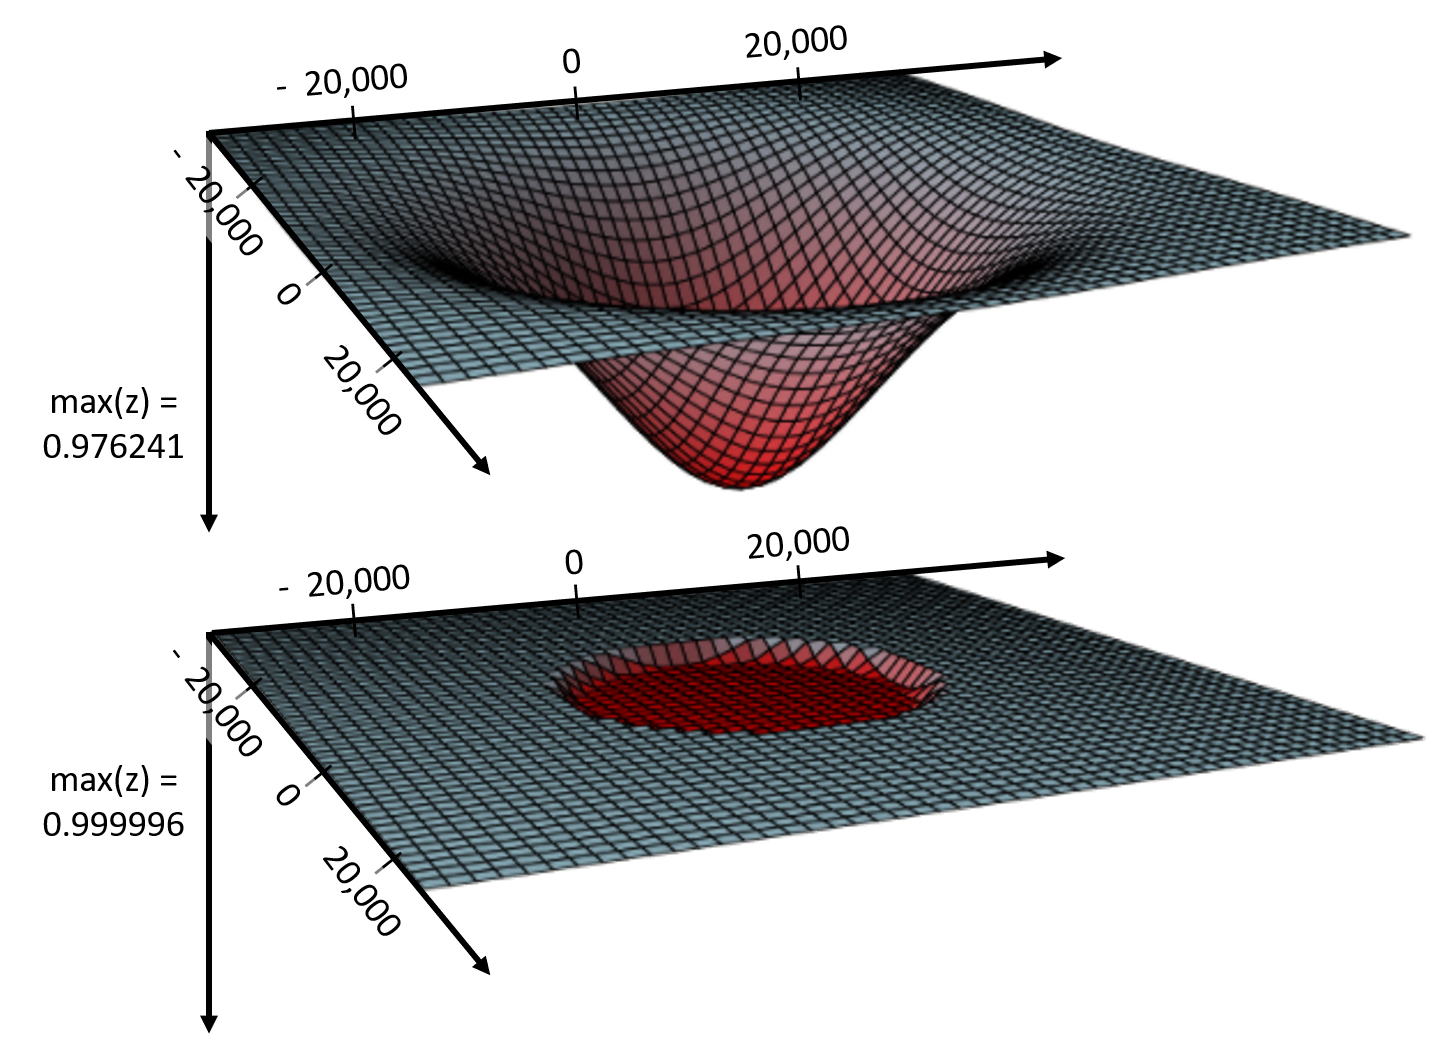
\includegraphics[width=0.9\textwidth]{figures/theoretical_footprint.png}
\caption{\label{fig:theoretical_footprint} The theoretical footprint of a tourist and a private cabin.}
\end{figure}

Despite the lower theoretical footprint of private cabins, their sheer number leads to a larger potential footprint ($6311 km^2$) than the one of tourist cabins ($4737 km^2$) in our study area. However, the realized footprint of tourist cabins ($956 km^2$) is larger than the one of private cabins ($781 km^2$), due to the larger overlap between the potential footprint of tourist cabins with the suitable habitat for reindeer (see Figure~\ref{fig:empirical_footprint}. 

And the resulting loss of suitability habitat for reindeer is: 50 \%  and 39 \% for respectively private and tourist cabins (using the `natural' suitability as the reference). Not surprisingly these percentages drop to 48 \% and 37 \% for respectively private and tourist cabins, when we consider the added effect on top of the other infrastructures.

\begin{sidewaysfigure}
    \centering
    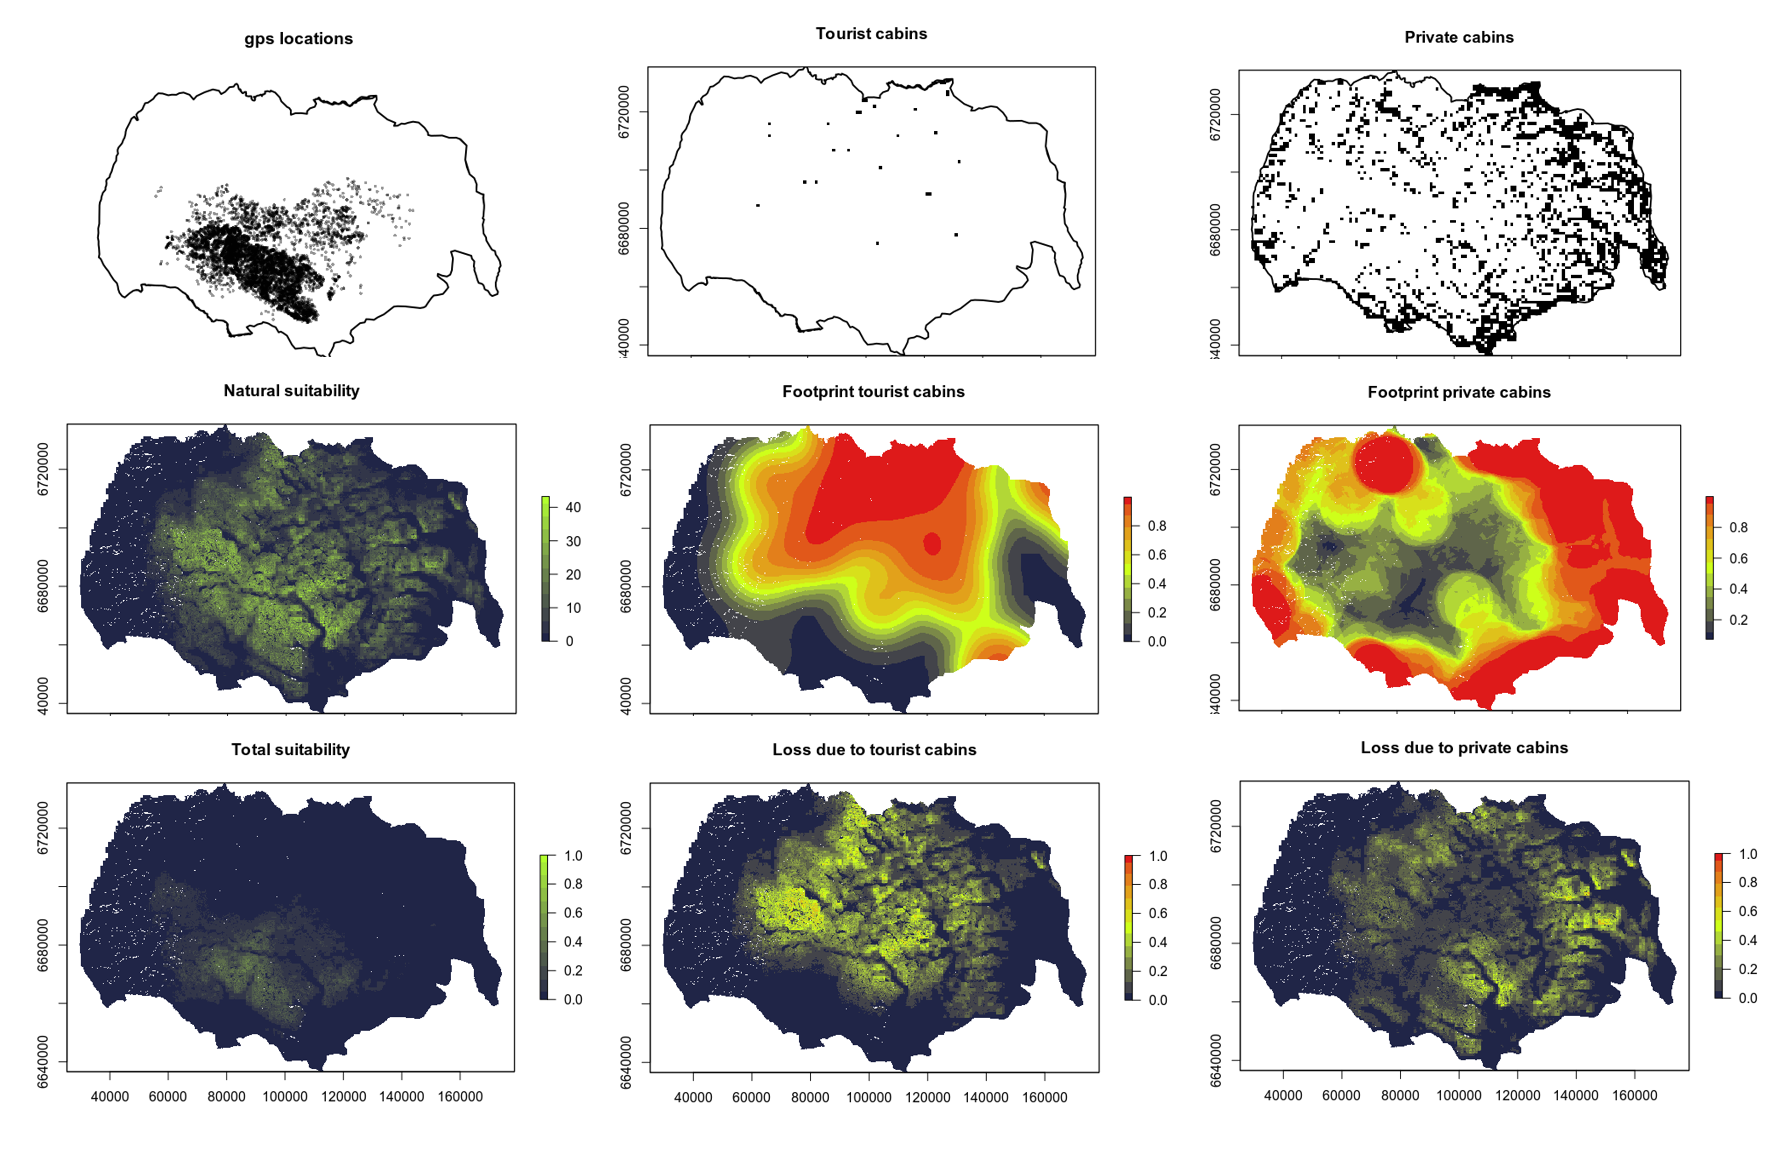
\includegraphics[width=1.0\textwidth]{figures/empirical_footprint.png}
    \caption{\label{fig:empirical_footprint} The empirical and realized footprint of tourist and private cabins in our study area. }
\end{sidewaysfigure}


\section{Discussion}

In this study we developed a methodology to quantify the cumulative impacts of multiple features, which we applied to the quantification of different types of anthropogenic footprints of infrastructures. We applied this methodology to quantify the effect of private and public cabins on the space use of a wild reindeer population in Norway. We found evidence for cumulative effects from multiple features on reindeer space use. In other words, reindeer not only responded to the nearest cabin, but also cabins further away. 

Studies quantifying the ZoI most commonly focus on the distance to the nearest feature of an infrastructure. We developed an approach using 'density' calculations in a GIS to estimate simultaneously the ZoI and the cumulative effect size of multiple features of an infrastructure. Whereas the approach of focusing only on the nearest feature assumes that the additional effect of any further features is zero, our approach assumes that the additional effect of each feature is identical, while accounting for the ZoI of these features. Our demonstration shows that the later is a more realistic assumption for the effects of cabins on wild reindeer, we did not address potential interactions or diminishing effects of additional features. More complex modeling frameworks would need to be developed to allow for such effects. 

We found marked differences in the size of the footprint depending upon the type of footprint. While the structural footprint of a single cabin will not be dramatically different between public and private cabins, we found that the functional theoretical footprint of a public cabin was substantially larger than the one of a private cabin, both due to its larger ZoI and its larger effect size. We used the footprint concept as a way to integrate the effects of the ZoI and the effect size into a single metric. The ZoI and effect size correspond in the footprint metaphor to respectively the size of the foot and the weight it carriers. Although the theoretical footprint of private cabins was smaller, their potential footprint was much larger than the one of public cabins, due to their sheer number ( 13,015 private vs. 26 public cabins). However, the placement of these public cabins in more suitable reindeer habitat resulted in a larger loss of habitat and therefore a larger realized footprint than for private cabins. In the footprint metaphor, the imprint on the habitat suitability corresponds to the softness of the substrate; the imprint even of a heavy foot will be small on a hard substrate (i.e. unsuitable habitat), whereas even a light foot may leave a strong imprint on a soft substrate (i.e. suitable habitat). Given the different components contributing to the realized footprint of an infrastructure on ecosystems cautions against a singular focus on its structural footprint.   
While our study addresses cumulative impacts of different features of an infrastructure, different types of cumulative impacts can be considered. Our approach can readily be extended to address the cumulative impact of different types of infrastructures. For instance, in our case study the cumulative realized footprint of both public and private cabins on reindeer space use was XXX (compared to the impact of either public or private cabins: XXX and XXX respectively). However, cumulative impacts can also originate from effects on different functions. For instance, an infrastructure, such as a road, may affect space use due to reduced use of the area surrounding the road resulting in habitat loss, but also lead to habitat fragmentation due to a barrier effect on movements \citep{beyer2016you}. The extension of the concepts developed in this study to other cumulative effects will prove an important avenue for future research.

For demonstrative purposes we kept the model relatively simple and reindeer space use is affect by many other human infrastructures, such as roads, trails, etc. \citep[e.g.][]{panzacchi2015searching}. For instance, the very large ZoI ($20 km$) we found for public cabins is likely driven by the trail network associated to this type of cabins. Thus, the anthropogenic footprint of cabins on reindeer space use identified in this study are the combined effects of these cabins with the associated infrastructures. 

In summary, the framework we developed to quantify the cumulative impacts of infrastructures and its anthropogenic footprint will contribute to the further development of the methodological basis for environmental impact studies. In particular, it allows us to quantify the effects of 'nibbling' on ecosystems, which presents a major challenge to land planners in the context of ecological sustainability. Each individual infrastructure may have a small impact, but collectively they lead to important loss of habitat.



\bibliographystyle{apalike}
\bibliography{bibliography}


\end{document}
